\begin{figure}[t]
    \centering
    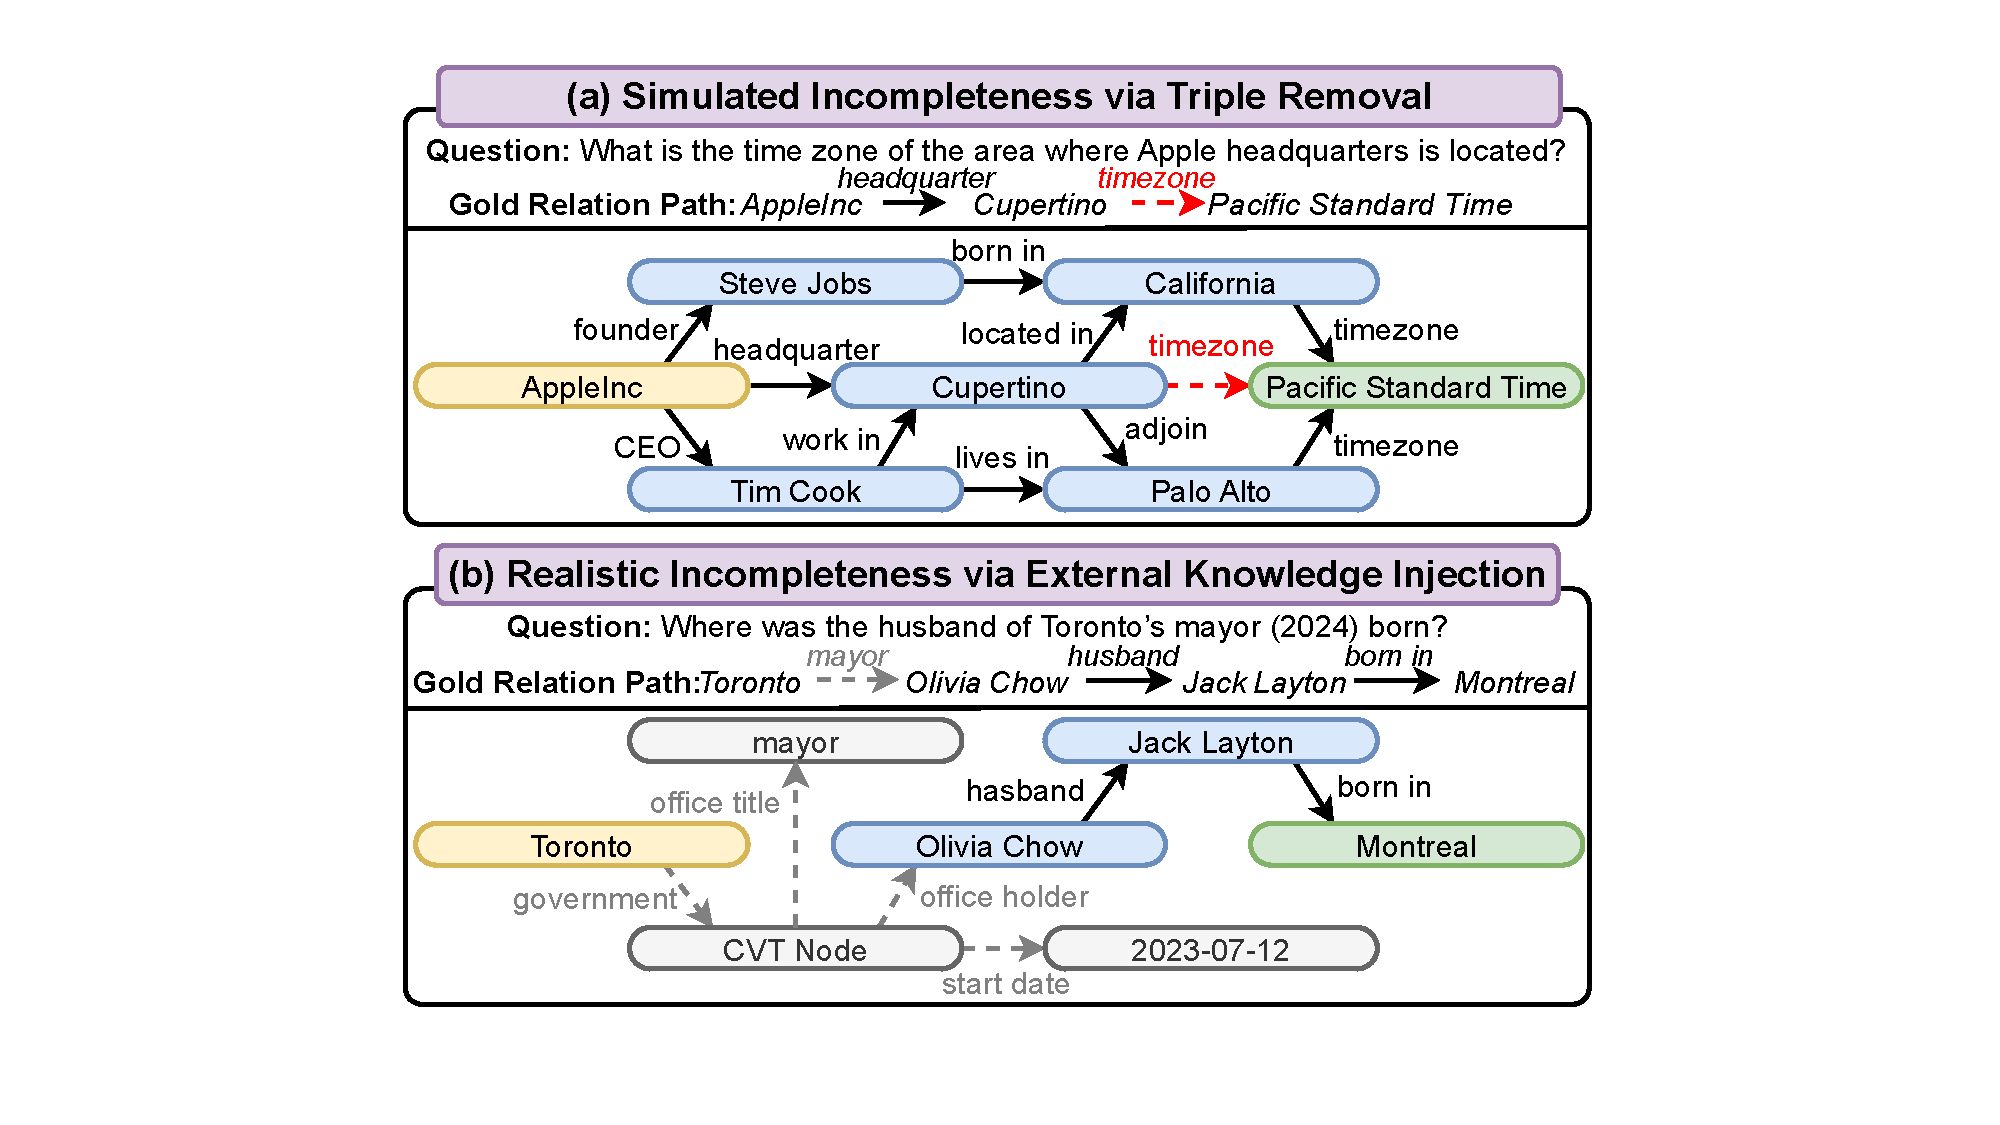
\includegraphics[width=\linewidth]{figures/figure_0.pdf}
    \caption{Illustration of two strategies for constructing incomplete KG scenarios. (a) Simulated incompleteness by removing triples from the KG; red dashed arrows denote the deleted facts. (b) Realistic incompleteness by incorporating external knowledge; gray dashed arrows indicate newly introduced information. CVT (Compound Value Type) nodes are used to represent multi-entity relations in Freebase.}
    \label{fig:IKG_Construction}
\end{figure}
